% Conditional outcome distributions, with the lecture's expectation notation.
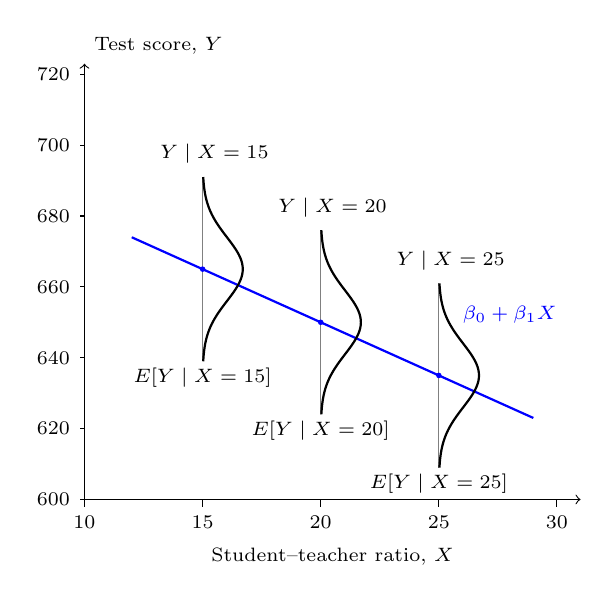
\begin{tikzpicture}[x=0.30cm,y=0.045cm,font=\scriptsize]
\draw[->] (10,600)--(31,600);
\node[below] at (20.5,589) {Student--teacher ratio, $X$};
\draw[->] (10,600)--(10,723) node[above right]{Test score, $Y$};
\foreach \x in {10,15,20,25,30}
  \draw (\x,600)--(\x,598) node[below]{\x};
\foreach \y in {600,620,640,660,680,700,720}
  \draw (10,\y)--(9.8,\y) node[left]{\y};
\draw[blue,thick] (12,674)--(29,623);
\foreach \x/\m in {15/665,20/650,25/635}{
  \draw[gray] (\x,\m-26)--(\x,\m+26);
  \draw[thick,domain=-26:26,samples=65,variable=\t]
    plot ({\x+1.7*exp(-\t*\t/162)},{\m+\t});
  \fill[blue] (\x,\m) circle (1pt);
  \node[above,align=center] at (\x+0.5,\m+27)
    {$Y\mid X=\x$};
  \node[below,fill=white,inner sep=1pt] at (\x,\m-27)
    {$\mathbb{E}[Y\mid X=\x]$};
}
\node[above,blue] at (28,647) {$\beta_0+\beta_1X$};
\end{tikzpicture}
